\chapter{Communication and Protocol}
\label{ch:communication-protocol}

This chapter describes the communication model underlying a GlobalPlatform-like
environment.  It focuses on how commands are expressed, transported and
secured, and how they enable the deployment and administration of applications.

This organization reflects the architectural role of communication in
GlobalPlatform: APDUs provide the transport abstraction, GlobalPlatform
commands define the management semantics, and secure channels enforce the
security properties of these operations.

%--------------------------------------------------
\section{APDU Model}

Application Protocol Data Units (APDUs) provide the fundamental communication
abstraction between an off-card entity and the platform. In the present
document, they are not introduced as a low-level transport artifact, but as the
basic interaction unit on top of which GlobalPlatform defines its management
protocol. An APDU carries a command or a response in a compact and structured
form, while the actual management semantics is defined at a higher level by the
command set interpreted by the platform. In other words, APDUs define the shape
of the exchange, not yet its business meaning. The GlobalPlatform Card
specification relies on this separation: commands are exchanged as APDUs, while
their interpretation depends on the instruction code, the class byte, and the
current execution context. \gpref{gp-card}{§9.4, §11}

\begin{figure}[ht]
  \centering
  \begin{tikzpicture}[
    field/.style={
      draw,
      rounded corners=2pt,
      minimum height=1cm,
      align=center,
      font=\small
    },
    lab/.style={font=\footnotesize},
    >=Latex
  ]
    % Command APDU
    \node[lab] at (-5.9,3.25) {\textbf{Command APDU}};
    \node[field, minimum width=1.2cm] (cla) at (-4.8,0) {CLA};
    \node[field, minimum width=1.2cm] (ins) at (-3.4,0) {INS};
    \node[field, minimum width=1.2cm] (p1)  at (-2.0,0) {P1};
    \node[field, minimum width=1.2cm] (p2)  at (-0.6,0) {P2};
    \node[field, minimum width=1.4cm] (lc)  at (1.0,0) {Lc};
    \node[field, minimum width=3.0cm] (data) at (3.6,0) {Data};
    \node[field, minimum width=1.4cm] (le)  at (6.2,0) {Le};

    % Response APDU
    \node[lab] at (-5.4,-2.15) {\textbf{Response APDU}};
    \node[field, minimum width=7.2cm] (rdata) at (0.2,-3.2) {Response Data};
    \node[field, minimum width=1.2cm] (sw1) at (4.7,-3.2) {SW1};
    \node[field, minimum width=1.2cm] (sw2) at (6.1,-3.2) {SW2};

    % Annotations
    \draw[->] (cla.north) -- ++(0,1.65) node[above,align=center,font=\footnotesize] {Class byte:\\routing and protection context};
    \draw[->] (ins.north) -- ++(0,1.15) node[above,align=center,font=\footnotesize] {Instruction code};
    \draw[->] (p1.north) -- ++(0,0.65) node[above,align=left,font=\footnotesize] {Parameters};
    \draw[->] (p2.north) -- ++(0,0.65);
    \draw[->] (data.south) -- ++(0,-0.65) node[below,align=center,font=\footnotesize] {Command payload};
    \draw[->] (sw1.south) -- ++(0,-0.65) node[below,align=left,font=\footnotesize] {Status bytes};
    \draw[->] (sw2.south) -- ++(0,-0.65);

  \end{tikzpicture}
  \caption{Abstract structure of a command/response APDU pair.}
  \label{fig:apdu-abstract}
\end{figure}

Figure~\ref{fig:apdu-abstract} presents the abstract command/response structure
used throughout this document. A command APDU starts with a four-byte header
formed by the class byte (\texttt{CLA}), the instruction byte (\texttt{INS}),
and two parameter bytes (\texttt{P1}, \texttt{P2}). It may then contain a
length field (\texttt{Lc}), a data field, and an expected response length
(\texttt{Le}). The response APDU mirrors this model in a simpler form: it
returns an optional response data field followed by two status bytes
\texttt{SW1} and \texttt{SW2}, which indicate success or failure and sometimes
encode additional protocol information. This abstract view is sufficient to
understand the role of APDUs in GlobalPlatform: they provide a generic and
extensible envelope for all management operations.  \gpref{gp-card}{§9.4}
\gpref{iso7816-4}{§5, §6}

\subsection{APDU Vocabulary}

The APDU-related vocabulary used throughout this document is the
following:

\begin{itemize}
\item \textbf{command APDU}: an APDU sent by the interface device
  towards the secure element;
\item \textbf{response APDU}: an APDU returned by the secure element;
\item \textbf{header}: the four command bytes \texttt{CLA},
  \texttt{INS}, \texttt{P1}, and \texttt{P2};
\item \textbf{incoming data} or \textbf{command payload}: the bytes
  carried from the interface device to the secure element, logically measured by
  \texttt{Lc};
\item \textbf{outgoing data} or \textbf{response payload}: the bytes
  returned by the secure element before the final status, logically measured by
  \texttt{Le};
\item \textbf{status word}: the two-byte trailer \texttt{SW1/SW2};
\item \textbf{logical APDU case}: one of the four abstract APDU shapes
  (Case~1 to Case~4), independent of the concrete transport protocol;
\item \textbf{\texttt{T=0} transport}: the half-duplex,
  character-oriented transport defined by ISO/IEC~7816-3;
\item \textbf{deferred response}: the \texttt{T=0} realization of a
  logical Case~4 exchange, where response data is announced by
  \texttt{61xx} and later recovered through \texttt{GET RESPONSE};
\item \textbf{ATR}: the \emph{Answer To Reset}, i.e. the first byte
  string emitted by the secure element after activation/reset and before the APDU
  command stream starts.
\end{itemize}

\subsection{APDU Cases under T=0}

Before considering GlobalPlatform command semantics, it is useful to
distinguish the four abstract command cases that arise from the presence
or absence of incoming and outgoing data. In the short-APDU model used
throughout this document, these cases are:

\begin{itemize}
\item \textbf{Case 1 (empty)}: the command carries only the four-byte
  header and no data is exchanged beyond the final status word;
\item \textbf{Case 2 (out)}: the command carries an expected response
  length \texttt{Le}, and the secure element returns response data followed by
  \texttt{SW1/SW2};
\item \textbf{Case 3 (in)}: the command carries a command length
  \texttt{Lc} and an incoming data field, but no response data beyond
  the final status word;
\item \textbf{Case 4 (in+out)}: the command carries incoming data and
  also logically expects response data.
\end{itemize}

At the abstract APDU level, these four cases are sufficient to describe
the shape of the exchange. Their concrete serialization depends on the
transport protocol. In particular, the classical \texttt{T=0} transport
is half-duplex and does not simply carry incoming and outgoing payloads
as a single full-duplex frame. As a result, a logical ``in+out'' APDU is
usually realized in two steps: the command first transfers its incoming
payload, and if response bytes are then available, the secure element indicates
this through a status word of the form \texttt{61xx}. The interface
device must
then issue a dedicated \texttt{GET RESPONSE} command to fetch the
pending outgoing bytes.

This is the key distinction between the abstract APDU model and its
\texttt{T=0} realization. Abstractly, Case~4 remains a single command
that both consumes and produces data. Concretely, the response payload
may be deferred and retrieved by one or more \texttt{GET RESPONSE}
commands. In the classical short-\texttt{T=0} convention, pending
response bytes are announced through a status word of the form
\texttt{61xx}, and the interface device then issues \texttt{GET RESPONSE}
(\texttt{INS = C0}, conventionally with \texttt{P1 = 00} and
\texttt{P2 = 00}) to retrieve the remaining bytes.

A command that only receives data typically terminates with a final
status word, while a command that only sends data can return its payload
immediately before that final status. A logical Case~4 command is
therefore the only case that needs this extra \texttt{GET RESPONSE}
step in a \texttt{T=0} exchange. This distinction also explains why the
fifth command byte cannot be interpreted in isolation: depending on the
case, it denotes either \texttt{Lc} or \texttt{Le}.

\subsubsection{Procedure bytes and immediate status}
\label{sec:apdu-t0-procedure-bytes}

After the interface device has transmitted the five-byte command
header, it does not interpret subsequent bytes as response data
immediately. It first waits for a \texttt{T=0} procedure byte. The
following values determine the next phase of the exchange:

\begin{itemize}
\item \texttt{INS} acknowledges transfer of all remaining command or
  response data bytes;
\item the one's complement of \texttt{INS} acknowledges transfer of
  exactly one data byte;
\item \texttt{60} is the NULL procedure byte: no data is transferred
  and the interface device continues waiting;
\item a valid \texttt{SW1} value terminates the command immediately,
  and the next byte is interpreted as \texttt{SW2}.
\end{itemize}

Consequently, a secure element may reject a command directly after its
header, for example with \texttt{69 85}, without first returning the
number of bytes announced by \texttt{Le}. There is no ambiguity with
response data: response bytes are interpreted as data only after an
\texttt{INS} or complemented-\texttt{INS} ACK has opened the data
transfer phase. Once that phase is open, the interface device counts the
announced bytes before interpreting the final \texttt{SW1/SW2}.

This byte-level multiplexing constrains instruction coding. For a
command transported over \texttt{T=0}, \texttt{INS} shall not be in
\texttt{60--6F} or \texttt{90--9F}, because these ranges are reserved
for NULL, status, and related procedure-byte meanings. Oxide SE command
definitions and Rustlet applications intended for the \texttt{T=0}
interface must respect this restriction. Appendix~\ref{app:apdu-over-t0}
describes how the reference implementation realizes these
procedure-byte transitions.

A concrete serialization depends on the underlying transport case. In the
classical \texttt{T=0} model, command and response exchanges are constrained by
a byte-oriented half-duplex protocol, and the APDU structure is materialized
through a small number of normalized cases depending on the presence or absence
of data and expected response bytes.  For the purpose of this chapter, the
important point is not the detailed enumeration of those cases, but the fact
that the abstract APDU model remains stable across transport variants: the same
logical command still consists of a header, optional command data, and a
structured response.

The detailed implementation strategy of APDU transport, including the mapping
of the abstract model to the \texttt{T=0} protocol, is discussed in
Chapter~8 (Reference Implementation), Section~\ref{sec:impl-apdu-t0}
according to \gpref{gp-card}{§5.3, §9.4}. The same transport principles
remain relevant even when higher-level services such as secure messaging
later wrap the command payload.

\subsection{Reference Smart-Card Link and Serial-Line Adaptation}
\label{sec:apdu-serial-adaptation}

In the ISO/IEC~7816 reference architecture, APDUs transported with
\texttt{T=0} cross the dedicated electrical interface of a contact smart card.
The contact assignment and physical interface are specified by
ISO/IEC~7816-2, while activation, ATR exchange, character framing, timing, and
the \texttt{T=0} transmission protocol are specified by ISO/IEC~7816-3
\cite{iso7816-2,iso7816-3}. This smart-card link is therefore more than an
ordinary serial port, even though \texttt{T=0} itself is a byte-oriented,
half-duplex protocol.

Most general-purpose microcontrollers available as off-the-shelf development
boards do not expose that complete smart-card electrical form factor. To make
oXiDe SE directly usable on such hardware, the reference implementation carries
the \texttt{T=0} byte exchange over a conventional serial line. This is a
deliberate transport adaptation: it preserves the APDU command/response model,
procedure bytes, ATR, and deferred-response behavior needed by the software,
but it does not claim that a UART connection is the ISO/IEC~7816 physical
interface.

Support for the actual ISO/IEC~7816 contact interface remains a reference
porting target. The kernel architecture must consequently keep APDU and
\texttt{T=0} processing independent of the serial-line driver, so that a board
providing the required smart-card peripheral and electrical interface can
replace the UART transport without changing GlobalPlatform command handling,
secure-channel processing, or Rustlet dispatch.

\subsection{Timing Constraints of the \texttt{T=0} Exchange}
\label{sec:apdu-t0-timing}

ISO/IEC~7816 should be read here as a layered set of constraints rather
than as a single monolithic APDU document:

\begin{itemize}
\item ISO/IEC~7816-1 defines the physical card characteristics
  \cite{iso7816-1};
\item ISO/IEC~7816-2 defines the contacts and their placement
  \cite{iso7816-2};
\item ISO/IEC~7816-3 defines activation/reset, the ATR, the elementary
  time unit, character framing, guard times, waiting times, and the
  \texttt{T=0} half-duplex character transport \cite{iso7816-3};
\item ISO/IEC~7816-4 defines the APDU model, command-response
  structure, logical channels, and commands such as
  \texttt{GET RESPONSE} \cite{iso7816-4}.
\end{itemize}

For the timing points that matter to an implementation,
ISO/IEC~7816-3 is the critical standard. ISO/IEC~7816-4 then explains
the logical APDU consequences of those transport constraints.

The first timing constraint appears during activation. Public summaries
of ISO/IEC~7816-3 restate that, after clock startup and reset
assertion, the secure element must emit its ATR within a bounded clock-cycle
window: the ATR begins between 400 and 40\,000 clock cycles after the
reset event \cite{adi-smartcard-fundamentals}. This is why the standard
budget is better understood in cycles than in milliseconds. At
2~MHz, 40\,000 cycles correspond to 20~ms; at higher clock rates, the
same normatively-defined window becomes shorter in wall-clock time.

The next important point is what happens \emph{after} the ATR. The
standardized transport does not grant a millisecond-scale software pause
between the end of the ATR and the start of the next command. On the
contrary, once the ATR is complete, the secure element waits for interface-device
characters under the active transmission parameters
\cite{iso7816-3}. The timing unit is the elementary time unit
(\emph{etu}), which ISO/IEC~7816-3 defines from the transmission
parameters and the secure-element clock. Public hardware documentation also
emphasizes the same operational view: the ETU is the bit clock, a
character frame is ten bits long, and guard/wait times are also
expressed in ETUs rather than in milliseconds
\cite{microchip-iso7816-usart,microchip-guardtime}.

This has a direct implementation consequence. At default settings, the
transport leaves only the normal character pause and guard-time budget
between adjacent protocol events. In practical terms, the hot
boundaries are:

\begin{itemize}
\item the end of ATR transmission and the beginning of the first command
  reception;
\item the end of command-header reception and the beginning of incoming
  payload reception for a logical Case~3 or Case~4 exchange;
\item the end of a status-word transmission and the beginning of the
  next command reception;
\item in a deferred Case~4 exchange, the end of a \texttt{61xx}
  transmission and the beginning of the next \texttt{GET RESPONSE}
  command.
\end{itemize}

The standard also constrains the opposite side of the timing problem:
characters emitted by the secure element are subject to waiting-time limits, so long
processing excursions before a required transmission are also
protocol-sensitive \cite{iso7816-3}. The important architectural point
is therefore not merely that \texttt{T=0} is synchronous in a
``schoolbook'' sense, but that its safety margins are intentionally
small and expressed at the byte/character level.

In the current prototype, the UARTs are not physically clocked by the
ISO card clock, so the exact hardware coupling differs from a literal
contact-card implementation. Nevertheless, the software consequence is
the same: these boundaries must be treated as hot-path transitions, and
implementers should avoid inserting logging, allocation, registry work,
or any other unrelated code between transmission completion and the next
receive step. Chapter~8 returns to this point and explains how the
current implementation keeps these transitions intentionally tight
(\S\ref{sec:impl-apdu-t0}).

Among the APDU header fields, the instruction byte \texttt{INS} carries the
first level of semantic meaning. It identifies the command family to be
executed, such as \texttt{INSTALL}, \texttt{LOAD}, \texttt{DELETE}, or
\texttt{GET STATUS} in the GlobalPlatform management model. In that sense,
\texttt{INS} is best understood as an opcode: it says \emph{what kind of
operation is requested}. However, \texttt{INS} alone is not enough to determine
the full meaning of a command. The detailed interpretation also depends on the
class byte, on the parameter bytes, and on the security context in which the
command is received. This is why APDUs should not be viewed as self-describing
business messages: they are compact protocol objects whose meaning emerges from
the combination of several header fields and from the current platform state.
\gpref{gp-card}{§11}

The class byte \texttt{CLA} is more subtle and, in practice, more informative
than a simple ``protocol class'' tag. In a GlobalPlatform setting, it plays at
least three distinct roles.  First, it distinguishes command spaces, in
particular whether the command is interpreted as an ISO-style command or as a
GlobalPlatform management command. The specification explicitly uses
ranges of \texttt{CLA} values to discriminate these cases. Second, the class
byte carries the logical channel number, in accordance with ISO/IEC~7816-4.
GlobalPlatform states that logical channel information shall be indicated in
the class byte of the command header, so the same instruction may be sent on
different channels, each channel being associated with a different selected
application or execution context. Third, the class byte is also used to
indicate whether secure messaging is applied to the command. In particular,
GlobalPlatform secure channel mechanisms modify the class byte to signal that
the APDU is protected, while the exact bit pattern depends on the logical
channel encoding and on the secure messaging mode.  \gpref{gp-card}{§9.4,
§11.3} \gpref{scp03}{§7}

The logical channel mechanism is important because it separates communication
contexts without changing the command vocabulary itself. A command is still
identified by its instruction code, but the \texttt{CLA} byte specifies on
which logical channel it is sent. From an architectural point of view, this
means that the APDU model already contains a lightweight routing mechanism: the
off-card entity does not only request an operation, it also addresses the
execution context in which this operation must be interpreted. This is
particularly relevant when several applications or management contexts coexist
on the same secure element. The GlobalPlatform Card Specification therefore treats the
logical channel information carried by \texttt{CLA} as part of the command
dispatching context. \gpref{gp-card}{§9.4}

The same byte also supports secure messaging. When a Secure Channel is active,
a command APDU is no longer a plain protocol object: it becomes a protected
message whose header and payload must be interpreted together with the
cryptographic context of the session. In SCP03, for example, the command header
is modified so that the class byte indicates that secure messaging is present;
the command may then include a command MAC and, depending on the requested
security level, encrypted command data. The specification also explains how
this marking interacts with logical channel information. Thus, the \texttt{CLA}
byte should be understood as the place where routing information and protection
state meet: it tells the platform both \emph{where} the command is addressed
and \emph{whether} it is protected. \gpref{gp-card}{§9.4} \gpref{scp03}{§7.1}

The APDU model is deliberately generic: its structure is stable and compact,
but most of the management meaning is not encoded in the shape of the message
itself. Instead, that meaning is reconstructed from three layers of
interpretation: the abstract APDU format, the command semantics associated with
the GlobalPlatform instruction set, and the security context associated with
secure messaging.  This separation is precisely what makes APDUs a suitable
foundation for a GlobalPlatform-like environment: they are generic enough to
transport very different commands, yet structured enough to support routing,
session protection, and administration semantics within a single uniform model.

From an implementation perspective, this layered interpretation of APDUs
directly translates into distinct software components. The concrete design
choices for parsing, dispatching and secure channel integration are discussed
in Chapter~8 (Reference Implementation).

%--------------------------------------------------
\section{GlobalPlatform Command Model}

GlobalPlatform defines a set of card management commands that give semantic
meaning to APDU exchanges. These commands are used to deploy, configure, manage
and query applications hosted on the platform. They are specified in the
GlobalPlatform Card Specification, which defines both their semantics and their
encoding within the APDU structure \gpref{gp-card}{§11, §11.9}.

Unlike the APDU model, which only defines a generic communication structure,
the GlobalPlatform command model defines a protocol of orchestration. Each
command corresponds to a well-defined operation on the internal state of the
secure element, such as loading executable content, installing an application,
managing keys or querying the registry. The specification explicitly organizes
these commands as \emph{card management commands}, executed under the authority
of a Security Domain \gpref{gp-card}{§7, §11}.

An important property of this model is that commands operate on opaque
payloads. GlobalPlatform does not define the binary format of applications;
instead, it defines how such binaries are transported, installed and managed
through sequences of APDUs. In particular, the loading process is defined as a
sequence of \texttt{LOAD} commands followed by \texttt{INSTALL} operations,
independently of the internal structure of the code being deployed
\gpref{gp-card}{§11.6, §11.7}.

Commands are not always used in isolation but are often composed into
higher-level workflows aligned with the application lifecycle. For instance,
application deployment typically involves secure channel establishment,
load-file loading, application installation and activation. These flows are implicitly
defined by the specification through command preconditions and state
transitions \gpref{gp-card}{§9, §11}.

From an architectural perspective, the command model also defines a separation
between identification, authorization and execution. Commands are addressed to
a given context (through the APDU model), executed under a Security Domain, and
validated against privilege and lifecycle constraints defined by the platform
\gpref{gp-card}{§7, §9.6}.

The detailed implementation of command parsing, dispatch, validation and
execution policies is out of scope of this chapter and is described in
Chapter~8 (Reference Implementation), Section~\ref{sec:impl-apdu-dispatch}.

\subsection{Command Overview}

The GlobalPlatform management model defines a set of APDU-based commands
used to control the lifecycle of applications, manage cryptographic material,
and interact with the internal state of the secure element. These commands are
specified in the GlobalPlatform Card Specification and are collectively
referred to as \emph{card management commands} \gpref{gp-card}{§11}.

From an architectural perspective, these commands can be grouped into several
categories according to their role in the system.

\paragraph{Application and Load File Lifecycle Management}

These commands are used to deploy, install, activate and remove application
code:

\begin{itemize}
\item \textbf{LOAD}: Transfers executable content (typically in multiple
    fragments) to the secure element.
\item \textbf{INSTALL}: Creates and configures application instances, and
    optionally makes them selectable.
\item \textbf{DELETE}: Removes application instances or load files from the secure
    element.
\item \textbf{SET STATUS}: Updates the lifecycle state of applications or
    Security Domains.
\item \textbf{GET STATUS}: Retrieves information about installed entities and
    their states.
\end{itemize}

These commands define the operational workflow of application deployment and
lifecycle management \gpref{gp-card}{§11.6, §11.7, §11.9} described in
Chapter~8, Section~\ref{sec:impl-lifecycle}.

\paragraph{Security and Key Management}

These commands manage cryptographic material and secure communication:

\begin{itemize}
\item \textbf{PUT KEY}: Installs or updates cryptographic keys within a
    Security Domain.
\item \textbf{INITIALIZE UPDATE}: Initiates a secure channel session.
\item \textbf{EXTERNAL AUTHENTICATE}: Completes the establishment of a secure
    channel.
\end{itemize}

They are central to enforcing authenticity and confidentiality of management
operations \gpref{gp-card}{§9.6, §11.8} \gpref{scp03}{§6} detailed in
Chapter~8, Section~\ref{sec:impl-scp}.

\paragraph{Data Management and Configuration}

These commands provide controlled access to internal data structures:

\begin{itemize}
\item \textbf{GET DATA}: Retrieves data objects from the secure element.
\item \textbf{STORE DATA}: Sends application-specific or platform-specific
    configuration data.
\end{itemize}

They enable controlled interaction with the internal registry and application
parameters \gpref{gp-card}{§11.4, §11.5} handled as described in Chapter~8,
Section~\ref{sec:impl-registry}.

\paragraph{Context and Communication Management}

These commands control the execution context and communication channels:

\begin{itemize}
\item \textbf{SELECT}: Selects an application or Security Domain as the current
    context.
\item \textbf{MANAGE CHANNEL}: Opens or closes logical communication channels.
\end{itemize}

They define how commands are routed and interpreted within the platform
\gpref{gp-card}{§9.4} see Chapter~8, Section~\ref{sec:impl-channel}.

\medskip

Although each command has a well-defined individual semantics, they are rarely
used in isolation. Instead, they are composed into structured sequences that
implement higher-level operations. For instance, application deployment
typically involves secure channel establishment, followed by a sequence of
\texttt{LOAD} commands, and completed by an \texttt{INSTALL} command.

From a design perspective, these commands form a minimal but expressive
instruction set that allows external entities to drive the evolution of the
platform state without requiring any knowledge of the internal representation
of applications. The command model therefore acts as a stable control interface
between the external management environment and the internal execution
platform.

The concrete implementation of command grouping, sequencing constraints and
state validation mechanisms is described in Chapter~8 (Reference
Implementation), Section~\ref{sec:impl-apdu-dispatch}.

\subsection{LOAD Command}

The \texttt{LOAD} command is used to transfer executable content to the
secure element. It is part of the application deployment process and is typically
followed by an \texttt{INSTALL} command. The semantics of this command are
defined in the GlobalPlatform Card Specification \gpref{gp-card}{§11.6}.

\apdudesc
{80}
{E8}
{last-block flag}
{\#block}
{var}
{00}
{Load File Data Block fragment}
{none}

Unlike most other commands, \texttt{LOAD} is designed to handle large payloads
that cannot fit within a single APDU. As a result, the loading process is
performed through a sequence of \texttt{LOAD} commands, each carrying a
fragment of the executable content.

The \texttt{P1} parameter indicates whether the current block is the last one
(bit~8), while \texttt{P2} carries the block number. This allows the secure
element to reconstruct the full load file incrementally.

The concatenated payload contains a Load File Data Block, normally a
\texttt{C4} BER-TLV object whose value is the executable load file. The
executable value remains opaque to GlobalPlatform: the specification defines
its transport envelope and sequence, not the implementation-specific binary
format carried inside it.

The \texttt{LOAD} command is therefore not an atomic operation but part of a
higher-level transactional process. The platform must ensure that partial or
inconsistent loading sequences do not result in a corrupted state. In
particular, the complete sequence must be validated before the loaded content
becomes usable.

On success, the secure element returns status word \texttt{90 00}. Other status values
may indicate:
\begin{itemize}
\item \texttt{6A80}: invalid data (malformed fragment)
\item \texttt{6985}: conditions not satisfied (e.g., missing secure channel)
\item \texttt{6A84}: insufficient memory
\item \texttt{6581}: memory failure
\end{itemize}

The handling of fragmentation, buffering, integrity checks, and
transactional guarantees remains implementation-dependent. It is
described in Chapter~8 (Reference Implementation),
Section~\ref{sec:impl-load}.

\subsection{INSTALL Command}
\label{sec:gp-install-command}

The \texttt{INSTALL} command is used to create, configure and optionally
activate an application instance on the secure element. It is the central
operation that completes the application deployment process after the transfer
of executable content through \texttt{LOAD} commands. Its semantics are defined
in the GlobalPlatform Card Specification \gpref{gp-card}{§11.7}.

\apdudesc
{80}
{E6}
{mode}
{flags}
{var}
{00}
{AIDs and installation parameters}
{none}

Unlike \texttt{LOAD}, which is concerned with data transfer, \texttt{INSTALL}
operates at the level of the platform state. It binds previously loaded
executable content to an application instance, associates identifiers, defines
privileges and establishes the execution context.

The \texttt{P1} parameter specifies the installation mode. Depending on its
value, the command may perform different operations such as installation for
load, installation for install, installation for make selectable, or a
combination of these. This makes \texttt{INSTALL} a polymorphic command whose
behavior depends on control flags rather than a single fixed semantics.

The payload contains several identifiers, including:
\begin{itemize}
\item the Executable Load File AID
\item the application (or instance) AID
\item the Security Domain AID under which the application is installed
\item optional installation parameters
\end{itemize}

These elements define how the application is registered and under which
authority it operates. The interpretation of installation parameters is left to
the execution environment and is not specified by GlobalPlatform.

The \texttt{INSTALL} command also plays a critical role in privilege
assignment. It is through this command that an application may be granted
specific capabilities, such as delegated management rights or access to secure
services. These privileges are enforced by the Security Domain model
\gpref{gp-card}{§7, §11.7}.

On success, the secure element returns status word \texttt{90 00}. Other status values
may indicate:
\begin{itemize}
\item \texttt{6A80}: invalid data (incorrect AID or parameters)
\item \texttt{6985}: conditions not satisfied (e.g., missing prerequisites)
\item \texttt{6982}: security status not satisfied
\item \texttt{6A84}: insufficient memory
\end{itemize}

From a protocol perspective, \texttt{INSTALL} terminates the loading sequence
and makes the application available to the platform, either immediately or
after an explicit lifecycle transition.

The detailed implementation of installation semantics, including registry
updates, privilege assignment and lifecycle transitions, is described in
Chapter~8 (Reference Implementation), Section~\ref{sec:impl-install}.

\subsection{DELETE Command}

The \texttt{DELETE} command is used to remove application instances or load
files from the secure element. It is part of the application lifecycle management and
complements the \texttt{LOAD} and \texttt{INSTALL} commands by enabling the
removal of previously deployed content. Its semantics are defined in the
GlobalPlatform Card Specification \gpref{gp-card}{§11.9}.

\apdudesc
{80}
{E4}
{00}
{flags}
{var}
{00}
{AID(s) to delete}
{none}

The command operates on one or more identifiers provided in the payload,
typically Application Identifiers (AIDs) corresponding to application instances,
load files, or Security Domains. \texttt{P1} is zero. Depending on the control
flags encoded in \texttt{P2}, the command may delete:
\begin{itemize}
\item a specific application instance
\item a complete load file (including all associated instances)
\item a Security Domain and its subordinate hierarchy through cumulative deletion
\end{itemize}

Unlike \texttt{INSTALL}, which introduces new state, \texttt{DELETE} removes
entries from the internal registry and releases associated resources such as
memory and identifiers.

The operation is subject to strict constraints. In particular:
\begin{itemize}
\item an application cannot be deleted while it is selected on another
      logical channel
\item a load file cannot be removed if dependent applications still exist
\item appropriate privileges must be held by the invoking Security Domain
\end{itemize}

These constraints ensure the consistency of the platform state and prevent
partial or inconsistent removal operations.

On success, the secure element returns status word \texttt{90 00}. Other status values
may indicate:
\begin{itemize}
\item \texttt{6A88}: referenced data not found
\item \texttt{6985}: conditions not satisfied
\item \texttt{6982}: security status not satisfied
\item \texttt{6A84}: not enough memory or resources to complete the operation
\end{itemize}

From an architectural perspective, \texttt{DELETE} is a destructive operation
that must preserve system integrity. It requires validation of dependencies and
enforcement of lifecycle constraints before state modification.

The detailed implementation of dependency checking, registry updates and
resource cleanup is described in Chapter~8 (Reference Implementation),
Section~\ref{sec:impl-delete}.

\subsection{SET STATUS Command}

The \texttt{SET STATUS} command is used to update the lifecycle state of an
object managed by the platform, such as an application, a load file or a
Security Domain. It plays a key role in controlling the activation and
deactivation of components. Its semantics are defined in the GlobalPlatform
Card Specification \gpref{gp-card}{§11.9}.

\apdudesc
{80}
{F0}
{type}
{state}
{var}
{00}
{AID of target object}
{none}

The command operates on a target object identified by its AID, provided in the
payload.  The \texttt{P1} parameter specifies the type of object being
addressed, while the \texttt{P2} parameter encodes the state-control operation.
The Oxide SE reference profile accepts:

\begin{center}
\begin{tabular}{p{0.20\textwidth}p{0.52\textwidth}}
\textbf{Field value} & \textbf{Meaning} \\
\hline
\texttt{P1 = 20} & package / executable load-file object; \\
\texttt{P1 = 40} & ordinary application instance; \\
\texttt{P1 = 80} & Security Domain instance; \\
\texttt{P2 = 80} & lock the addressed object; \\
\texttt{P2 = 00} & unlock the addressed object into its usable state.
\end{tabular}
\end{center}

Typical lifecycle states depend on the object family and on the selected
platform profile. The Oxide SE lifecycle subset used by the reference model is
defined in Section~\ref{sec:gp-lifecycle-model}: packages are
\emph{Loaded} or \emph{Locked}, application instances and Security Domains are
\emph{Selectable} or \emph{Locked}, and key objects are \emph{Active} or
\emph{Locked}. \texttt{SET STATUS} controls packages, application instances,
and Security Domains. Key-object lifecycle is controlled by key-management
commands, not by \texttt{SET STATUS}.

The different object types manipulated by the platform, as well as their
associated attributes, are defined in Section~\ref{sec:gp-object-model}. Their
lifecycle states and valid transitions are described in
Section~\ref{sec:gp-lifecycle-model}.

Lifecycle transitions are not arbitrary. The platform enforces a state machine
that restricts valid transitions and ensures consistency. For example, a locked
package cannot be instantiated, a locked application cannot be selected, and a
locked Security Domain cannot be used to establish a secure channel.

The execution of \texttt{SET STATUS} is subject to strict access control. Only
authorized Security Domains holding the appropriate privileges may modify
lifecycle states \gpref{gp-card}{§7, §11.9}.
Oxide SE additionally applies the following reference policy: the target
object must be under the authority of the Security Domain used for the command;
protected commands use the Security Domain bound to the active secure channel;
clear commands use the root Security Domain and are accepted only when that
Security Domain explicitly allows \texttt{SET STATUS} without SCP. The
development \texttt{NullSecurityDomain} allows this bypass; production
Security Domains do not.

On success, the secure element returns status word \texttt{90 00}. Other status values
may indicate:
\begin{itemize}
\item \texttt{6A80}: invalid parameters (unsupported state transition)
\item \texttt{6985}: conditions not satisfied
\item \texttt{6982}: security status not satisfied
\end{itemize}

From an architectural perspective, \texttt{SET STATUS} is a control command
that governs the visibility and usability of objects without modifying their
underlying content.

The detailed implementation of lifecycle state machines and transition
validation is described in Chapter~8 (Reference Implementation),
Section~\ref{sec:impl-lifecycle}.

\subsection{GET DATA Discovery Objects}
\label{sec:gp-get-data-discovery}

Before opening a secure channel, a host must be able to discover the
administrative protocols offered by the selected Security Domain. The
GlobalPlatform discovery path uses \texttt{GET DATA}; it does not require the
host to probe establishment commands until one happens to succeed
\gpref{gp-card}{§11.3, §11.4}.

\apdudesc
{80}
{CA}
{tag high}
{tag low}
{00}
{var}
{none}
{requested data object}

\paragraph{Card Recognition Data: tag \texttt{0066}.}

The response is a BER-TLV object \texttt{66} containing a Card Recognition
Data template \texttt{73}. Its minimum useful GlobalPlatform structure is:

\begin{verbatim}
66 LL
   73 LL
      06 07 2A 86 48 86 FC 6B 01
      60 0B 06 09 2A 86 48 86 FC 6B 02 02 03
      63 09 06 07 2A 86 48 86 FC 6B 03
      64 0B 06 09 2A 86 48 86 FC 6B 04 scp i
      ...
\end{verbatim}

The first three OIDs identify the GlobalPlatform recognition authority, the
Card Specification version, and the card-identification scheme. Each
\texttt{64} template then advertises one Secure Channel Protocol through the
OID \texttt{\{globalPlatform 4 scp i\}}. Several \texttt{64} templates may be
present. For the Oxide SE profile:

\begin{itemize}
\item SCP03 is identified by \texttt{scp = 03}; \texttt{i = 00} advertises
      S8 and \texttt{i = 01} advertises S16, using random challenges and
      without a separately initiated R-MAC session;
\item SCP11 is identified by \texttt{scp = 11}; \texttt{i} is a bitmap whose
      bits select SCP11a, SCP11b and SCP11c, with bit~7 set for the S16
      profile. Therefore SCP11a+c is advertised as \texttt{i = 51}, and
      SCP11a+b+c as \texttt{i = 53}.
\end{itemize}

An Issuer Security Domain intended for production shall advertise the SCPs it
actually accepts. A development-only authority that implements no secure
channel may return the same well-formed recognition structure without a
\texttt{64} template. A supplementary Security Domain may also include its
\texttt{73} recognition data in the proprietary part of its \texttt{SELECT}
response; \texttt{GET DATA 0066} remains the explicit discovery command.

\paragraph{Card Capability Information: tag \texttt{0067}.}

The optional object \texttt{67} provides more detailed capabilities. Each
supported SCP is represented by an \texttt{A0} template:

\begin{verbatim}
67 LL
   A0 LL 80 01 scp 81 LL i... [82 LL supported-key-bitmap]
   ...
   82 03 privilege-bytes
   83 01 load-file-data-block-hash
\end{verbatim}

Tag \texttt{80} identifies the SCP, tag \texttt{81} lists its supported
parameter values, and the SCP03-specific tag \texttt{82} identifies supported
static key types. The outer tag \texttt{82} reports the three-byte application
privilege model and tag \texttt{83} reports the Load File Data Block Hash
algorithm. Absence of this optional data object is reported as
\texttt{6A88}; it must not be replaced by invented capabilities.

The implementation-side construction of these objects is described in
Chapter~8, Section~\ref{sec:impl-gp-discovery}.

\subsection{GET STATUS Command}

The \texttt{GET STATUS} command is used to retrieve information about objects
managed by the platform, such as applications, load files and Security Domains.
It provides a structured view of the internal registry and is essential for
platform introspection. Its semantics are defined in the GlobalPlatform Card
Specification \gpref{gp-card}{§11.9}.

\apdudesc
{80}
{F2}
{object family}
{continuation/format}
{var}
{00}
{\texttt{4F} AID criterion, optional \texttt{5C}}
{\texttt{E3} status records}

\texttt{P1} selects the object family:

\begin{center}
\begin{tabular}{p{0.18\textwidth}p{0.60\textwidth}}
\textbf{P1} & \textbf{Objects requested} \\
\hline
\texttt{80} & Issuer Security Domain; \\
\texttt{40} & applications and supplementary Security Domains; \\
\texttt{20} & executable load files; \\
\texttt{10} & executable load files and their modules.
\end{tabular}
\end{center}

The modern TLV response format sets \texttt{P2.b2}. A first request therefore
uses \texttt{P2 = 02}; if the response ends with \texttt{63 10}, the host sends
the same query with \texttt{P2 = 03} to request the next occurrence. The
command data starts with a mandatory \texttt{4F} search criterion. Its value
may be empty, an exact AID, or an AID prefix. An optional \texttt{5C} tag list
may request particular response fields.

Each returned object is a constructed \texttt{E3} record. Its mandatory and
family-specific fields include:
\begin{itemize}
\item \texttt{4F}: object AID;
\item \texttt{9F70}: lifecycle state;
\item \texttt{C5}: three-byte privileges for an application or Security
      Domain;
\item \texttt{C4}: executable-module or package association when applicable;
\item \texttt{CC}: associated Security Domain;
\item \texttt{84}: module AID for the load-file-and-modules query.
\end{itemize}

The \texttt{GET STATUS} command is a read-only operation but is still subject
to access control. An authority sees only objects associated directly or
indirectly with its Security Domain hierarchy. In oXiDe SE the Global Registry
form is recognized only at the technical-root APDU boundary and invokes this
same lookup with the root as authority; no privilege bit bypasses subtree
filtering. Keys and private data objects are not registry status entries
exposed by this command.

On success, the secure element returns status word \texttt{90 00} along with the response
data.  Other status values may indicate:
\begin{itemize}
\item \texttt{63 10}: more matching records are available;
\item \texttt{6A88}: no matching object found
\item \texttt{6982}: security status not satisfied
\item \texttt{6A86}: incorrect \texttt{P1}/\texttt{P2}
\item \texttt{6A80}: malformed query data
\end{itemize}

From an architectural perspective, \texttt{GET STATUS} exposes a controlled
view of the internal state of the platform. It allows external entities to
observe the system without modifying it, and is therefore complementary to
lifecycle management commands.

The detailed implementation of registry traversal, filtering and response
encoding is described in Chapter~8 (Reference Implementation),
Section~\ref{sec:impl-get-status}.

\subsection{PUT KEY Command}

The \texttt{PUT KEY} command is used to install or update cryptographic keys within a
Security Domain. It is a central mechanism for managing the secure channel infrastructure
and enforcing cryptographic policies on the platform. Its semantics are defined in the
GlobalPlatform Card Specification \gpref{gp-card}{§11.8}.

\apdudesc
{80}
{D8}
{old key ver./chain}
{id./multiple}
{var}
{00}
{key data and attributes}
{none}

The command allows the caller to introduce new keys or replace existing ones. These keys
are typically used for secure channel establishment (e.g., SCP02 or SCP03), but may also
serve other platform-level cryptographic purposes.

The low seven bits of \texttt{P1} identify the key version being replaced (zero
when adding a key); bit~8 indicates whether another \texttt{PUT KEY} command
follows in the same operation. The low seven bits of \texttt{P2} identify the
first key, and bit~8 indicates that the command data contains several
consecutively numbered keys. The command data begins with the new key version,
then encodes each key's type, length, material and key-check value.

The payload contains the key material and associated attributes. Depending on the context,
the key data may be:
\begin{itemize}
\item encrypted under a key encryption key (KEK)
\item diversified based on secure-element-specific parameters
\item accompanied by metadata such as key type and length
\end{itemize}

The execution of \texttt{PUT KEY} is restricted to authorized Security Domains holding
appropriate privileges. Improper use of this command may compromise the entire security
model, as it directly affects the trust anchors of the platform.

On success, the secure element returns status word \texttt{90 00}. Other status values may indicate:
\begin{itemize}
\item \texttt{6A80}: invalid key data
\item \texttt{6985}: conditions not satisfied
\item \texttt{6982}: security status not satisfied
\item \texttt{6A88}: referenced key not found
\end{itemize}

From an architectural perspective, \texttt{PUT KEY} is not only a configuration command but
also a root-of-trust management operation. It defines the cryptographic material used to
protect all subsequent communications.

The detailed implementation of key storage, versioning, diversification and secure
handling is described in Chapter~8 (Reference Implementation),
Section~\ref{sec:impl-key-management}.

\subsection{INITIALIZE UPDATE Command}

The \texttt{INITIALIZE UPDATE} command initiates the establishment of a Secure
Channel between the host and the secure element. It is the first step of the
mutual authentication protocol defined by GlobalPlatform and is typically
followed by the \texttt{EXTERNAL AUTHENTICATE} command. Its behavior is
specified in the GlobalPlatform Card Specification and the Secure Channel
Protocol specifications \gpref{gp-card}{§9.6} \gpref{scp03}{§6}.

\apdudesc
{80}
{50}
{key ver.}
{00}
{08}
{var}
{host challenge (8 bytes)}
{card challenge and security data}

The command is sent by the host to request cryptographic material required to
derive session keys. It contains a host-generated random value, known as the
\emph{host challenge}, typically 8 bytes long.

Upon reception, the secure element responds with a structured payload that
includes:
\begin{itemize}
\item a fresh card challenge (random or pseudorandom value generated by the secure element)
\item key diversification data (if applicable)
\item a key version number identifying the key set in use
\item cryptographic data used to authenticate the card
\end{itemize}

This exchange allows both parties to derive a shared set of session keys, based
on:
\begin{itemize}
\item pre-shared static keys (installed via \texttt{PUT KEY})
\item exchanged random challenges (host and card)
\item optional diversification data
\end{itemize}

At this stage, the Secure Channel is not yet fully established. The host must
verify the authenticity of the card using the received cryptographic data, and
then complete the protocol using the \texttt{EXTERNAL AUTHENTICATE} command.

The response payload is structured but depends on the Secure Channel Protocol
in use (e.g., SCP02 or SCP03). GlobalPlatform defines the format of this data,
but its detailed interpretation is protocol-specific \gpref{scp03}{§6.2}.

On success, the secure element returns status word \texttt{90 00} along with the response
data.  Other status values may indicate:
\begin{itemize}
\item \texttt{6700}: incorrect host-challenge length
\item \texttt{6985}: conditions not satisfied
\item \texttt{6982}: security status not satisfied
\item \texttt{6A88}: key set not found
\end{itemize}

From an architectural perspective, \texttt{INITIALIZE UPDATE} is not a
management command but a protocol bootstrap operation. It establishes the
cryptographic context required to protect subsequent APDU exchanges.

The detailed implementation of challenge generation, session key derivation and
response formatting is described in Chapter~8 (Reference Implementation),
Section~\ref{sec:impl-scp-init}.

\subsection{EXTERNAL AUTHENTICATE Command}

The \texttt{EXTERNAL AUTHENTICATE} command completes the establishment of a
Secure Channel following the \texttt{INITIALIZE UPDATE} command. It allows the
host to prove knowledge of the shared secret and to activate secure messaging
for subsequent exchanges. Its behavior is defined in the GlobalPlatform Card
Specification and Secure Channel Protocol specifications \gpref{gp-card}{§9.6}
\gpref{scp03}{§6.3}.

\apdudesc
{84}
{82}
{sec. lvl}
{00}
{10/20}
{absent}
{host cryptogram followed by the transmitted C-MAC}
{none}

The command contains a cryptographic value, known as the \emph{host
cryptogram}, computed by the host using the session keys derived from the
\texttt{INITIALIZE UPDATE} exchange.  This value allows the secure element to
authenticate the host.

SCP03 Amendment~D protects \texttt{EXTERNAL AUTHENTICATE} itself with a
command MAC. The class byte therefore carries the secure-messaging indication
(\texttt{84} on logical channel zero), and the command data is the
profile-sized host cryptogram followed by the transmitted C-MAC. For the S8
profile, \texttt{Lc = 10}: eight bytes of host cryptogram and eight bytes of
transmitted C-MAC. For the S16 profile, \texttt{Lc = 20}: sixteen bytes of host
cryptogram and sixteen bytes of transmitted C-MAC. The C-MAC is computed from
an all-zero initial chaining value over the command header, whose \texttt{Lc}
already includes the transmitted C-MAC length, followed by the host cryptogram.
The full sixteen-byte C-MAC becomes the initial command and response MAC
chaining value for subsequent secure messaging; S8 only truncates the value on
the wire.

The \texttt{P1} parameter encodes the requested SCP03 security level for the
session. GlobalPlatform defines the following values:
\begin{itemize}
\item \texttt{00}: no command or response secure messaging;
\item \texttt{01}: C-MAC;
\item \texttt{03}: C-MAC and C-ENC;
\item \texttt{11}: C-MAC and R-MAC;
\item \texttt{13}: C-MAC, C-ENC, and R-MAC;
\item \texttt{33}: C-MAC, C-ENC, R-MAC, and R-ENC.
\end{itemize}

This parameter determines how subsequent APDUs will be protected, including
whether their payload is authenticated and/or encrypted.

Upon reception, the secure element verifies the host cryptogram using its own
derivation of the session keys. If the verification succeeds, the Secure
Channel is established and the selected security level is activated. From this
point on, APDUs exchanged between the host and the secure element are wrapped according
to the secure messaging rules defined by the selected protocol.

If cryptographic authentication fails, the command is rejected with
\texttt{63 00} and the session is not established.

On success, the secure element returns status word \texttt{90 00}. Other status values
may indicate:
\begin{itemize}
\item \texttt{6300}: authentication failed
\item \texttt{6700}: incorrect authentication-data length
\item \texttt{6982}: security status not satisfied
\item \texttt{6985}: conditions not satisfied
\item \texttt{6A80}: invalid cryptographic data
\item \texttt{6A86}: unsupported security level or incorrect \texttt{P1/P2}
\end{itemize}

From an architectural perspective, \texttt{EXTERNAL AUTHENTICATE} marks the
transition from an unauthenticated communication state to a secure,
authenticated and optionally encrypted session. It effectively activates the
protection mechanisms that will apply to all subsequent commands.

The detailed implementation of cryptogram verification, session activation and
secure messaging enforcement is described in Chapter~8 (Reference
Implementation), Section~\ref{sec:impl-scp-auth}.

%--------------------------------------------------
\section{Secure Channel Protocol}
\label{sec:protocol-scp}

The Secure Channel Protocol (SCP) defines how APDU exchanges are protected in
terms of authenticity, integrity and confidentiality. In a GlobalPlatform
environment, SCP is not a transport protocol but a security layer applied on
top of the APDU model. Its purpose is to ensure that management commands are
executed only if they originate from an authenticated entity and have not been
modified in transit.

Several variants of SCP exist. The profiles relevant to this architecture are
SCP03, which is based on pre-shared AES keys, and the SCP11 family
(SCP11a/SCP11b/SCP11c), which uses elliptic-curve key agreement to establish
the symmetric keys later used by the same GlobalPlatform secure-messaging
grammar.

It is important to state explicitly that SCP03 is a \emph{symmetric}
secure-channel protocol. Its mutual authentication and secure messaging
mechanisms are built from pre-shared AES keys and do not require RSA, ECC, or
any other asymmetric primitive. This point is easy to blur because the wider
GlobalPlatform ecosystem also discusses transport of asymmetric keys and
certificate-related operations, but these are not part of the cryptographic
core of SCP03 itself. In fact, GlobalPlatform's compact IoT configuration
identifies a minimal profile centered on the Issuer Security Domain, AES, and
SCP03 only \cite{gp-compact-iot}.

From a protocol perspective, all Secure Channel profiles introduce three main
mechanisms:
\begin{itemize}
\item a profile-specific establishment sequence;
\item session-key derivation;
\item common secure messaging for command and response protection.
\end{itemize}

%--------------------------------------------------
\subsection{Official Establishment Commands}

GlobalPlatform secure-channel establishment is expressed through ordinary APDU
commands. The commands below are the protocol-level entry points that a
Security Domain uses to open or evolve a secure channel.

\texttt{INITIALIZE UPDATE} starts SCP03 establishment.

\apdudesc
{80}
{50}
{key ver.}
{00}
{08/10}
{var}
{host challenge}
{key data, card challenge, card cryptogram}

\texttt{EXTERNAL AUTHENTICATE} completes SCP03 establishment, authenticates
the host, and selects the requested secure-messaging level.

\apdudesc
{84}
{82}
{sec. lvl}
{00}
{10/20}
{absent}
{host cryptogram followed by the transmitted C-MAC}
{none}

\texttt{PERFORM SECURITY OPERATION} is used by SCP11a/SCP11c to submit and
verify OCE certificate material before the actual key-agreement APDU.

\apdudesc
{80}
{2A}
{key ver.}
{key id.}
{var}
{00}
{\texttt{CERT.OCE.ECKA} or related security-operation data}
{none}

The command returns \texttt{6600} when certificate verification fails,
\texttt{6A80} when the command data is malformed, \texttt{6A86} when the
reference-control parameters are invalid or select a profiled-out option, and
\texttt{6A88} when the referenced CA key is unavailable.

\texttt{MUTUAL AUTHENTICATE} opens SCP11a and SCP11c. Its command data is a
BER-TLV Control Reference Template with tag \texttt{A6}; its successful
response returns card public-key material and a receipt.

\apdudesc
{80}
{82}
{key ver.}
{key id.}
{var}
{var}
{\texttt{A6} CRT with SCP11 key-agreement parameters}
{\texttt{5F49} card key material and \texttt{86} receipt}

Both SCP11 mutual-authentication forms return \texttt{6A80} for malformed CRT
or public-key data, \texttt{6A88} when a referenced ECKA key or required
identity object cannot be resolved, and \texttt{6985} when a mandatory prior
step such as OCE certificate authentication has not completed.

The SCP11b internal-authentication command opens SCP11b. Its command shape is
similar to SCP11 mutual authentication, but the profile semantics are
different: the card authenticates itself to the OCE, while OCE authorization
is provided outside the SCP11b exchange.

\apdudesc
{80}
{88}
{key ver.}
{key id.}
{var}
{var}
{\texttt{A6} CRT with SCP11b key-agreement parameters}
{\texttt{5F49} card key material and \texttt{86} receipt}

The same \texttt{6A80}/\texttt{6A88} distinction applies to SCP11b internal
authentication: malformed cryptographic input is different from a referenced
key or identity object that is not present.

Once the channel is open, ordinary commands are sent as protected APDUs. The
instruction byte remains the instruction of the logical command
(\texttt{SELECT}, \texttt{INSTALL}, application command, and so on), while the
class byte carries the secure-messaging indication. Under GlobalPlatform
Amendment~D secure messaging, encrypted or clear command data is followed
directly by the C-MAC; response data is followed directly by the R-MAC when
response protection is active. The real response status remains the APDU
\texttt{SW1/SW2} trailer.

\apdudesc
{84}
{INS}
{P1}
{P2}
{var}
{var}
{protected command data followed by C-MAC}
{protected response data followed by R-MAC, then SW1/SW2}

There is no single universal ``close secure channel'' APDU in the base flow.
The active session is normally ended by reset, by logical-channel management,
or by starting a new establishment sequence for the same Security Domain and
channel. SCP03 profiles that use the optional explicit R-MAC session commands
are described in Section~\ref{sec:rmac-session-management}; those commands do
not apply to SCP11.

%--------------------------------------------------
\subsection{SCP03 Session Establishment}

SCP03 is established through the two-step handshake composed of
\texttt{INITIALIZE UPDATE} followed by \texttt{EXTERNAL AUTHENTICATE}
\gpref{scp03}{§6}.

The \texttt{INITIALIZE UPDATE} command allows the secure element to provide:
\begin{itemize}
\item a card challenge
\item key diversification data (optional)
\item a key version identifier
\item a card cryptogram
\end{itemize}

The host uses this information, together with pre-shared keys, to derive
session keys and to verify the authenticity of the card.

The \texttt{EXTERNAL AUTHENTICATE} command completes the protocol by sending a
host cryptogram, authenticating that cryptogram with the initial C-MAC, and
selecting a security level. If verification succeeds, the Secure Channel is
activated and all subsequent APDU exchanges may be protected. The initial
C-MAC starts from a sixteen-byte zero chaining value. The full sixteen-byte
result becomes the first secure-messaging chain value, even when the S8 profile
transmits only its first eight bytes.

The resulting session is attached to the Security Domain and logical channel
on which the establishment APDUs were exchanged. A representative SCP03
sequence is shown below. The byte-level derivation inputs and chaining rules
are detailed in Appendix~\ref{app:scp-data-objects}.

\begin{verbatim}
1. SELECT the Security Domain
   C-APDU: 00 A4 04 00 Lsd <SD-AID> 00
   R-APDU: <FCI> 90 00

2. INITIALIZE UPDATE
   C-APDU: 80 50 key-version 00 Lc <host challenge> 00
   R-APDU: <key data> <key info> <card challenge> <card cryptogram> 90 00

3. EXTERNAL AUTHENTICATE
   C-APDU: 84 82 security-level 00 Lc <host cryptogram> <C-MAC>
   R-APDU: 90 00

4. Protected command
   C-APDU: 84 INS P1 P2 Lc <data or encrypted data> <C-MAC> Le
   R-APDU: <data or encrypted data> <R-MAC> SW1 SW2
\end{verbatim}

%--------------------------------------------------
\subsection{Session Key Derivation}

Each Secure Channel establishment sequence produces session keys scoped to one
Security Domain session and one logical channel. SCP03 derives these keys from
pre-shared AES key material and host/card challenges. SCP11 derives them from
profile-specific ECC contributions and a profile-specific \texttt{SharedInfo}
structure. In both cases, the resulting keys are then consumed by the common
GlobalPlatform secure-messaging grammar.

The detailed SCP03 KDF inputs, SCP11 \texttt{SharedInfo} composition, key
usage qualifiers and cryptographic building blocks are collected in
Appendix~\ref{app:scp-data-objects}.\footnote{Keeping the derivation formats in
the appendix avoids duplicating profile tables in the main APDU chapter; the
normative point here is that establishment and protected messaging are two
separate protocol phases.}

%--------------------------------------------------
\subsection{SCP11 Session Establishment}

SCP11 is the asymmetric GlobalPlatform secure-channel family. Its
establishment APDUs differ by profile, but all three profiles derive symmetric
secure-messaging keys and then use the same protected-APDU grammar as SCP03.
The complete BER-TLV layout of the \texttt{A6} Control Reference Template,
profile bytes, identity material and example exchanges is given in
Appendix~\ref{app:scp-data-objects}.

\textbf{SCP11a} authenticates OCE key material before opening the channel with
\texttt{MUTUAL AUTHENTICATE}. The standard sequence is:
\texttt{SELECT} the Security Domain, optionally retrieve card certificate or
key material with \texttt{GET DATA}, submit \texttt{CERT.OCE.ECKA} with
\texttt{PERFORM SECURITY OPERATION}, then open the channel with
\texttt{MUTUAL AUTHENTICATE}.

\textbf{SCP11b} authenticates the card to the OCE and opens the channel with
\texttt{INTERNAL AUTHENTICATE}. OCE authorization is outside the SCP11b
exchange and must be supplied by the selected Security Domain policy.
Its standard sequence is: \texttt{SELECT} the Security Domain, optionally
retrieve card certificate or key material with \texttt{GET DATA}, perform the
external OCE authorization required by policy, then open the channel with
\texttt{INTERNAL AUTHENTICATE}.

\textbf{SCP11c} authenticates \texttt{CERT.OCE.ECKA} with
\texttt{PERFORM SECURITY OPERATION}, then opens the channel with
\texttt{MUTUAL AUTHENTICATE}. The card public-key material returned in
\texttt{5F49} is the material bound into the receipt calculation.
Its standard sequence is close to SCP11a at APDU level:
\texttt{SELECT}, optional \texttt{GET DATA}, \texttt{PERFORM SECURITY
OPERATION}, then \texttt{MUTUAL AUTHENTICATE}; the profile-specific
differences are in the authenticated material, receipt binding and
\texttt{SharedInfo} construction.

The \texttt{A6} CRT contains the SCP identifier, key-usage qualifier,
algorithm identifiers, requested key length, optional identity material, and
the OCE ephemeral public key. The detailed BER-TLV layout of this CRT and the
profile-specific SharedInfo rules are given in
Appendix~\ref{app:scp-data-objects}.

%--------------------------------------------------
\subsection{Secure Messaging}

Once the Secure Channel is established, APDU commands are no longer transmitted
in clear.  Instead, they are wrapped using secure messaging mechanisms.

This protection includes:
\begin{itemize}
\item command authentication (C-MAC)
\item optional command encryption (C-ENC)
\item optional response authentication (R-MAC)
\end{itemize}

At protocol level, wrapping an APDU involves:
\begin{itemize}
\item modifying the command header
\item optionally encrypting the command data with ISO9797-M2 padding
\item computing a chained C-MAC over the protected command representation and
      appending its transmitted bytes directly to the command data field
\item optionally encrypting the response data and appending the chained R-MAC
      directly to it; the actual response status bytes are included in the
      R-MAC input and remain the response APDU trailer
\end{itemize}

The response APDU may also include a response MAC, depending on the selected
security level.

\begin{figure}[p]
\centering
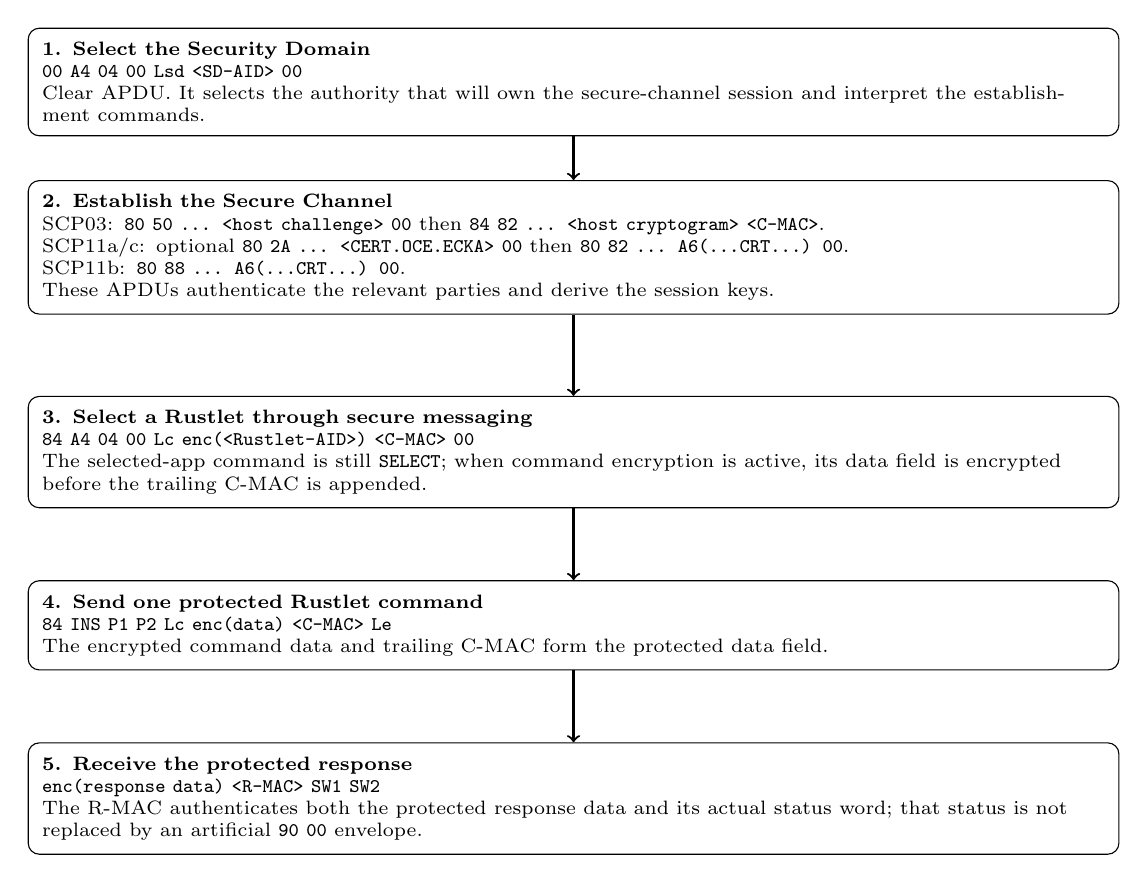
\begin{tikzpicture}[
    font=\scriptsize,
    scstep/.style={draw, rounded corners, align=left, text width=13.5cm,
                   inner sep=5pt},
    arrow/.style={->, thick}
]
\node[scstep] (s1) at (0,0) {
\textbf{1. Select the Security Domain}\\
\texttt{00 A4 04 00 Lsd <SD-AID> 00}\\
Clear APDU. It selects the authority that will own the secure-channel
session and interpret the establishment commands.
};

\node[scstep] (s2) at (0,-2.1) {
\textbf{2. Establish the Secure Channel}\\
SCP03: \texttt{80 50 ... <host challenge> 00}
then \texttt{84 82 ... <host cryptogram> <C-MAC>}.\\
SCP11a/c: optional \texttt{80 2A ... <CERT.OCE.ECKA> 00}
then \texttt{80 82 ... A6(...CRT...) 00}.\\
SCP11b: \texttt{80 88 ... A6(...CRT...) 00}.\\
These APDUs authenticate the relevant parties and derive the session keys.
};

\node[scstep] (s3) at (0,-4.7) {
\textbf{3. Select a Rustlet through secure messaging}\\
\texttt{84 A4 04 00 Lc enc(<Rustlet-AID>) <C-MAC> 00}\\
The selected-app command is still \texttt{SELECT}; when command encryption is
active, its data field is encrypted before the trailing C-MAC is appended.
};

\node[scstep] (s4) at (0,-6.9) {
\textbf{4. Send one protected Rustlet command}\\
\texttt{84 INS P1 P2 Lc enc(data) <C-MAC> Le}\\
The encrypted command data and trailing C-MAC form the protected data field.
};

\node[scstep] (s5) at (0,-9.1) {
\textbf{5. Receive the protected response}\\
\texttt{enc(response data) <R-MAC> SW1 SW2}\\
The R-MAC authenticates both the protected response data and its actual status
word; that status is not replaced by an artificial \texttt{90 00} envelope.
};

\draw[arrow] (s1) -- (s2);
\draw[arrow] (s2) -- (s3);
\draw[arrow] (s3) -- (s4);
\draw[arrow] (s4) -- (s5);
\end{tikzpicture}
\caption{Typical APDU flow from Security Domain selection to protected Rustlet command}
\label{fig:protected-rustlet-flow}
\end{figure}

%--------------------------------------------------
\subsection{CLA Encoding and Secure Messaging Indication}

The use of secure messaging is indicated directly in the APDU header, through
specific bits in the \texttt{CLA} byte.

In GlobalPlatform, the class byte encodes both:
\begin{itemize}
\item the logical channel number
\item the secure messaging status
\end{itemize}

When secure messaging is active, the \texttt{CLA} byte is modified to signal
that the APDU is protected. This affects how the command is interpreted by the
card:
\begin{itemize}
\item the payload must be unwrapped before processing
\item the MAC must be verified
\item the session state must be valid
\end{itemize}

This design ensures that secure messaging is orthogonal to the command
semantics: the same command (e.g., \texttt{INSTALL}) may be sent in clear or in
protected form, depending on the session state.

The exact encoding of secure messaging indicators within the \texttt{CLA} byte
is defined in the specification and must be handled consistently with logical
channel encoding \gpref{gp-card}{§9.4} \gpref{scp03}{§7}.

%--------------------------------------------------
\subsection{Operational Flow}

From a system perspective, the use of a Secure Channel follows a structured
sequence:

\begin{enumerate}
\item The host initiates the session using the protocol-specific establishment
      commands
\item The host authenticates using the protocol-specific authentication
      command(s)
\item The Secure Channel is established
\item Subsequent APDUs are transformed according to the common GlobalPlatform
      secure-messaging rules
\item The session remains active until explicitly terminated or reset
\end{enumerate}

This flow introduces a stateful layer on top of the APDU model, where the
interpretation of commands depends not only on their content but also on the
current session state.

\subsection{Protocol Invariants}

A conforming Secure Channel processing path must preserve the following
protocol invariants:

\begin{itemize}
\item session state is scoped to the selected Security Domain and logical
      channel;
\item session keys are used only within the session that derived them;
\item secure-messaging policy is enforced before command dispatch;
\item malformed protected APDUs, invalid MAC chains, stale receipts and replayed
      commands are rejected before their logical command is executed;
\item session invalidation prevents further use of the old MAC chain or old
      receipt material.
\end{itemize}

The implementation mapping of these invariants is described in Chapter~8
(Reference Implementation), Section~\ref{sec:impl-scp}.

\subsection{APDU Transformation under Secure Messaging}

Once the Secure Channel is established, APDU commands are no longer transmitted
in clear.  Instead, they are transformed through a wrapping process that
applies authentication and optional encryption to the command and response.

At a high level, the transformation operates as follows:
\begin{itemize}
\item the \texttt{CLA} byte is modified to indicate secure messaging
\item command data is optionally encrypted and the C-MAC is appended directly
      to the resulting data field
\item response data is optionally encrypted and the R-MAC is appended directly
      to it, before the actual \texttt{SW1/SW2}
\end{itemize}

This transformation preserves the logical structure of the APDU while modifying
its encoding and interpretation.
The precise binary ordering, padding, chaining and response-body shapes are
specified in Appendix~\ref{app:scp-data-objects}.

%--------------------------------------------------
\section{Secure Channel Extensions}

While Secure Channel Protocols define the core mechanisms required to protect
command APDUs, GlobalPlatform also specifies a set of extensions that enhance
the security model, in particular for response protection and advanced
messaging scenarios.

These extensions are not always mandatory but may be required depending on the
security policy of the deployment. At protocol level, they introduce additional
state and sequencing constraints that must be handled consistently with the
base SCP model.

%--------------------------------------------------
\subsection{Response Protection (R-MAC)}

The standard secure messaging model ensures the integrity and authenticity of
command APDUs.  However, responses returned by the secure element are not always
protected by default.

To address this limitation, GlobalPlatform defines a response protection
mechanism based on a Response Message Authentication Code (R-MAC). When
enabled, each response APDU includes a cryptographic MAC computed by the secure element
using the session key \texttt{S-RMAC} \gpref{scp03}{§6.2}.

This mechanism provides:
\begin{itemize}
\item integrity of response data
\item authentication of the secure element
\item protection against replay or modification of responses
\end{itemize}

Using R-MAC requires:
\begin{itemize}
\item maintaining a response MAC chaining state
\item computing and appending a MAC to each response
\item verifying this MAC on the host side
\end{itemize}

The detailed implementation of response MAC computation and verification is
described in Chapter~8 (Reference Implementation), Section~\ref{sec:impl-scp}.

\subsection{R-MAC Session Management}
\label{sec:rmac-session-management}

GlobalPlatform defines optional SCP03 commands to explicitly control the use
of response protection through R-MAC sessions. They are companion commands,
not part of the mandatory two-command SCP03 establishment sequence. SCP11 does
not support \texttt{BEGIN R-MAC SESSION} or \texttt{END R-MAC SESSION};
its response protection is selected directly by the key-usage qualifier in
the establishment CRT.

\apdudesc
{80}
{7A}
{00}
{00}
{00}
{00}
{none}
{none}

The \texttt{BEGIN R-MAC SESSION} command enables response protection for
subsequent APDUs.  Once activated, all responses returned by the secure element include
an R-MAC computed using the session key.

The command does not carry any payload and simply updates the session state.

On success, the secure element returns \texttt{90 00}. Failure may indicate:
\begin{itemize}
\item \texttt{6985}: conditions not satisfied
\item \texttt{6982}: security status not satisfied
\end{itemize}

\apdudesc
{80}
{78}
{00}
{00}
{00}
{00}
{none}
{none}

The \texttt{END R-MAC SESSION} command disables response protection.

After this command, response APDUs are no longer protected by an R-MAC,
although command protection (C-MAC, C-ENC) may still be active depending on the
session configuration.

This command restores a lighter communication mode while preserving the
established Secure Channel.

On success, the secure element returns \texttt{90 00}. Errors may include:
\begin{itemize}
\item \texttt{6985}: conditions not satisfied
\end{itemize}

\subsection{Secure Messaging Variants}

SCP03 supports multiple security levels that define how APDUs are protected.

These levels include:
\begin{itemize}
\item no protection
\item command authentication (C-MAC)
\item command authentication and encryption (C-MAC + C-ENC)
\item full protection including response authentication (R-MAC)
\end{itemize}

The selected security level is negotiated during the 
\texttt{EXTERNAL AUTHENTICATE} command and applies to all subsequent APDUs.

At protocol level, this implies that the APDU processing pipeline must be
capable of:
\begin{itemize}
\item selectively applying encryption
\item computing MACs
\item validating incoming MACs
\item handling different combinations of protection
\end{itemize}

This flexibility introduces additional complexity in the implementation, as all
combinations must be supported consistently.

\subsection{SCP Variants}

Several Secure Channel Protocol variants exist within GlobalPlatform, notably
SCP02 and SCP03.

SCP02 is based on legacy cryptographic primitives (DES/3DES), while SCP03
relies on AES and provides stronger security guarantees.

SCP03 is preferable to legacy DES-based SCP variants due to:
\begin{itemize}
\item improved security (AES-based)
\item simpler key derivation model
\item better resistance to known attacks
\end{itemize}

Supporting multiple SCP variants may be required for compatibility, but it
increases the protocol and certification surface. This document treats SCP03
and the SCP11 family as the reference profiles for the platform model.

%--------------------------------------------------
\subsection{Asymmetric and Post-Quantum Perspective}

Because the broader GlobalPlatform environment also handles certificates,
asymmetric keys, and delegated management artifacts, it is natural to ask
whether an SCP03 implementation must also embed asymmetric cryptography. The
answer is no: SCP03 itself does not require RSA, ECC, or post-quantum
asymmetric primitives. Its secure-channel core is fully symmetric and AES-based
\gpref{scp03}{§4, §6}.

This does not mean that asymmetric cryptography is irrelevant to the platform
as a whole. It means only that it belongs to other services: key transport
policies, certificate handling, platform attestation, application-specific
crypto services, or future secure-channel evolution. GlobalPlatform's own
discussion of crypto agility and hybrid migration highlights this distinction:
the current SCP03 core remains symmetric, while later evolutions may combine it
with stronger or more agile asymmetric layers \cite{gp-hybrid-crypto}.

If this project later introduces a minimal post-quantum asymmetric toolbox at
platform level, the most natural reference points are the NIST standards:
\begin{itemize}
\item ML-KEM for key encapsulation and shared-secret establishment
      \cite{fips203}
\item ML-DSA for general-purpose digital signatures \cite{fips204}
\item SLH-DSA as a stateless hash-based signature alternative \cite{fips205}
\end{itemize}

These algorithms are not required to implement SCP03. They should be viewed as
optional higher-level capabilities, introduced only if the platform later needs
public-key exchange, signatures, attestation, or hybrid migration strategies.
If such support is added, the dependency chain should also account for the
underlying SHA-3 and SHAKE primitives standardized by NIST \cite{fips202}.

%--------------------------------------------------
\section{oXiDe SE Beta Protocol Scope}
\label{sec:oxide-beta-protocol-scope}

The preceding sections state the protocol model against which oXiDe SE is
assessed. They must not be read as a claim that every optional GlobalPlatform
mechanism is already implemented. The beta reference implementation currently
supports short APDUs using its serial-line adaptation of \texttt{T=0}, the management-command subset
needed for Rustlet deployment and registry administration, SCP03 S8/S16 at
security levels \texttt{01} and \texttt{03} in the kernel-native Security
Domain, response-protecting SCP03 in the full Rustlet Security Domain, and the
implemented SCP11a, SCP11b, and SCP11c profiles.

The following mechanisms are deliberately outside the beta profile:
\begin{itemize}
\item legacy DES/TDEA-based SCP variants, including SCP02;
\item the optional SCP03 \texttt{BEGIN R-MAC SESSION} and
      \texttt{END R-MAC SESSION} commands;
\item SCP03 security levels \texttt{11}, \texttt{13}, and \texttt{33} in the
      deliberately smaller kernel-native Security Domain profile. The full
      Rustlet Security Domain provides the response-protecting path used by the
      beta test campaign.
\end{itemize}

Other mechanisms remain planned or incomplete rather than excluded from the
architecture. In particular, logical channels and \texttt{MANAGE CHANNEL} are
post-beta work. The beta also accepts only the management encodings exercised
by its declared profile: one complete BER-TLV object per \texttt{STORE DATA} command;
\texttt{INSTALL [for load]} and combined \texttt{INSTALL [for install and make
selectable]} with an empty token field; one final \texttt{PUT KEY} command with
the supported raw key types; and the documented registry/lifecycle subset.
Multi-command key updates, non-empty Tokens, DAPs, Receipts, key
diversification or wrapping, and the remaining optional management forms are
not yet implemented. Their absence is an implementation limitation, not a
reinterpretation of the commands defined by GlobalPlatform.

%--------------------------------------------------
\section{Discussion}

The previous sections introduced the communication model of a
GlobalPlatform-like environment by separating three concerns: the APDU
transport abstraction, the command semantics defined by the GlobalPlatform
instruction set, and the security layer provided by the Secure Channel
Protocol.

From an architectural perspective, this separation is not only conceptual but
directly maps to a software design. The platform can be understood as a system
that receives commands, interprets them according to its current state, and
produces responses. At the highest level, it behaves as a reactive system
driven by APDU inputs and generating APDU outputs.

\paragraph{A Layered Interpretation Model}

The processing of a command can be decomposed into three successive stages:

\begin{itemize}
\item \textbf{Transport layer (APDU parsing)}: decoding the structure of the
    incoming command (CLA, INS, P1, P2, payload), including logical channel
        routing.

\item \textbf{Security layer (SCP processing)}: verifying and removing secure
    messaging protection (MAC verification, decryption), and enforcing session
        validity.

\item \textbf{Semantic layer (command execution)}: interpreting the instruction
    and modifying the internal state of the platform accordingly.
\end{itemize}

These layers define a processing pipeline in which each stage transforms the
command before passing it to the next one. The reverse pipeline is applied when
constructing the response.

The detailed implementation of this pipeline is described in Chapter~8
(Reference Implementation), Sections~\ref{sec:impl-apdu-dispatch} and
\ref{sec:impl-scp}.

\paragraph{A State Machine View}

From the outside, the platform can be modeled as a state machine. Each incoming
APDU represents a transition request, whose validity and effect depend on the
current state of the system.

This state includes:
\begin{itemize}
\item the lifecycle state of managed objects (applications, load files,
    Security Domains)
\item the current selection context (logical channel and selected application)
\item the secure channel state (inactive, initialized, authenticated)
\end{itemize}

Commands such as \texttt{LOAD}, \texttt{INSTALL} or \texttt{SET STATUS} trigger
state transitions, while commands such as \texttt{GET STATUS} expose the
current state without modifying it.

The definition of managed objects and their lifecycle is provided in
Chapter~3, Sections~\ref{sec:gp-object-model} and \ref{sec:gp-lifecycle-model}.

\paragraph{An Interpreter Loop Perspective}

From the inside, the platform is naturally implemented as an interpreter loop:

\begin{enumerate}
\item receive an APDU command
\item parse and validate its structure
\item unwrap secure messaging if required
\item dispatch the command based on its instruction code
\item execute the corresponding handler
\item produce a response APDU
\item apply secure messaging to the response if required
\item return the response
\end{enumerate}

This loop provides a unifying view of the system, where each command is treated
as an instruction in a control interface. The GlobalPlatform command set can
thus be interpreted as a minimal instruction set driving the evolution of the
platform state.

The implementation of this interpreter loop is detailed in Chapter~8 (Reference
Implementation).

\paragraph{Freedom of Implementation}

An important property of the GlobalPlatform model is that it defines a protocol
of interaction rather than an execution model. In particular:

\begin{itemize}
\item the format of application binaries is not specified
\item the runtime environment is not constrained
\item the internal representation of objects is implementation-dependent
\end{itemize}

This leaves significant freedom to the implementer, while ensuring
interoperability at the protocol level. As a result, different platforms may
expose identical command interfaces while relying on very different internal
architectures.

\paragraph{Link with the Threat Model}

The architecture described above directly relates to the threat model
introduced earlier.  Each layer of the processing pipeline corresponds to a
security boundary:

\begin{itemize}
\item the APDU interface is exposed to external adversaries
\item the secure channel enforces authenticity and integrity of commands
\item the command execution layer must enforce isolation and lifecycle
    constraints
\end{itemize}

In particular, the interpreter loop must ensure that:
\begin{itemize}
\item no command can bypass security checks
\item malformed or malicious inputs are rejected early
\item state transitions remain consistent with the lifecycle model
\end{itemize}

This highlights the importance of a strict separation between parsing, security
enforcement and command execution, as well as the need for explicit validation
at each stage.

From this perspective, the GlobalPlatform model can be seen as a controlled
interface to a stateful system, where security relies on the correct
composition of protocol handling, cryptographic protection and state
management.
